%versi 2 (8-10-2016)
\chapter{Landasan Teori}
\label{chap:teori}

Pada bab ini akan dijelaskan dasar teori mengenai \textit{library} jsoup yang meliputi kelas-kelas Jsoup, Connection, Response, Document, Elements, dan Element. Akan dibahas pula Portal Akademik Mahasiswa, IFStudentPortal, SIA Models, dan panduan \textit{Android Design} yang meliputi Panduan Aksesibilitas dan panduan \textit{Material Design}.

\section{Portal Akademik Mahasiswa 2018}
Portal Akademik Mahasiswa adalah sistem informasi berbasis \textit{web} yang diperuntukan bagi mahasiswa untuk memperoleh informasi kegiatan akademik \cite{studentportalunpar}. Portal Akademik Mahasiswa dapat di akses melalui URL \url{https://www.studentportal.unpar.ac.id/}. Mahasiswa harus \textit{login} dengan email mahasiswa agar bisa mengakses dan menggunakan fitur-fitur yang tersedia.     

\begin{figure}[H]
	\centering
	
\includegraphics[scale=0.3]{DokumenSkripsi/Gambar/stupor.PNG}
	\caption{Tampilan halaman awal Portal Akademik Mahasiswa} 
	\label{fig:studpor_home}
\end{figure}
\subsection{Analisis Fitur Portal Akademik Mahasiswa 2018}
Pada sub-bab ini akan dijelaskan mengenai fitur-fitur yang ada di Portal Akademik Mahasiswa 2018
\begin{enumerate}
    \item \textit{Login} : 
    Untuk dapat menggunakan situs Portal Akademik Mahasiswa, mahasiswa harus \textit{login} menggunakan email \textit{student} mahasiswa.
    \begin{itemize}
			\item Nama: \textit{Login}
			\item Aktor: Mahasiswa
			\item Deskripsi: \textit{Login} ke Portal Akademik Mahasiswa 
			\item Kondisi awal: Mahasiswa adalah mahasiswa Universitas Katolik Parahyangan
			\item Kondisi akhir: Halaman utama Portal Akademik Mahasiswa ditampilkan 
			\item Skenario utama: \\ \\
        \begin{tabular}{|p{0.5cm} |p{6cm}| p{6cm}|}
        \hline
            No & Aksi Aktor &  Reaksi Sistem \\ \hline     
            1 & Mahasiswa mengakses situs Portal Akademik Mahasiswa & Sistem menampilkan halaman depan \\ \hline 
            2 & Mahasiswa menekan tombol \textit{login} & Sistem menampilkan halaman \textit{login}\\ \hline 
            3 & Mahasiswa mengisi email dan kata sandi lalu menekan tombol \textit{login} & Sistem melakukan pengecekan identitas \textit{login} \\ \hline 
            4 & & Jika login berhasil maka sistem akan menampilkan halaman utama Portal Akademik Mahasiswa\\ \hline 
        \end{tabular}
    \end{itemize}
    \begin{figure}[H]
				\centering
				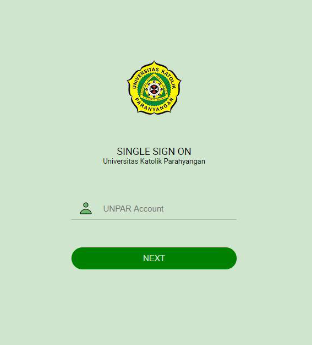
\includegraphics[scale=0.7]{Gambar/login_pam}
				\caption{Tampilan Login} 
				\label{fig:pam_login}
			\end{figure}
	\item \textit{FRS/PRS Daring} : 
    Mahasiswa dapat mengisi form rencana studi (FRS) atau melakukan perubahan rencana studi (PRS) secara daring di situs Portal Akademik Mahasiswa.
    \begin{itemize}
			\item Nama: FRS/PRS Daring
			\item Aktor: Mahasiswa
			\item Deskripsi: Mengisi form rencana studi (FRS) atau melakukan perubahan rencana studi (PRS) secara daring
			\item Kondisi awal: Mahasiswa sudah \textit{login} ke Portal Akademik Mahasiswa
			\item Kondisi akhir: Mahasiswa berhasil mengisi form rencana studi atau merubah rencana studi 
			\item Skenario utama: \\ \\
        \begin{tabular}{|p{0.5cm} |p{6cm}| p{6cm}|}
        \hline
            No & Aksi Aktor &  Reaksi Sistem \\ \hline     
            1 & Mahasiswa menekan tombol FRS/PRS & Sistem menampilkan halaman FRS/PRS \\ \hline 
            2 & Mahasiswa mengisi form rencana studi atau merubah rencana studi & \\ \hline 
            3 & Mahasiswa menekan tombol selesai & Sistem mencatat hasil FRS/PRS mahasiswa \\ \hline 
        \end{tabular}
    \end{itemize}
     \begin{figure}[H]
				\centering
				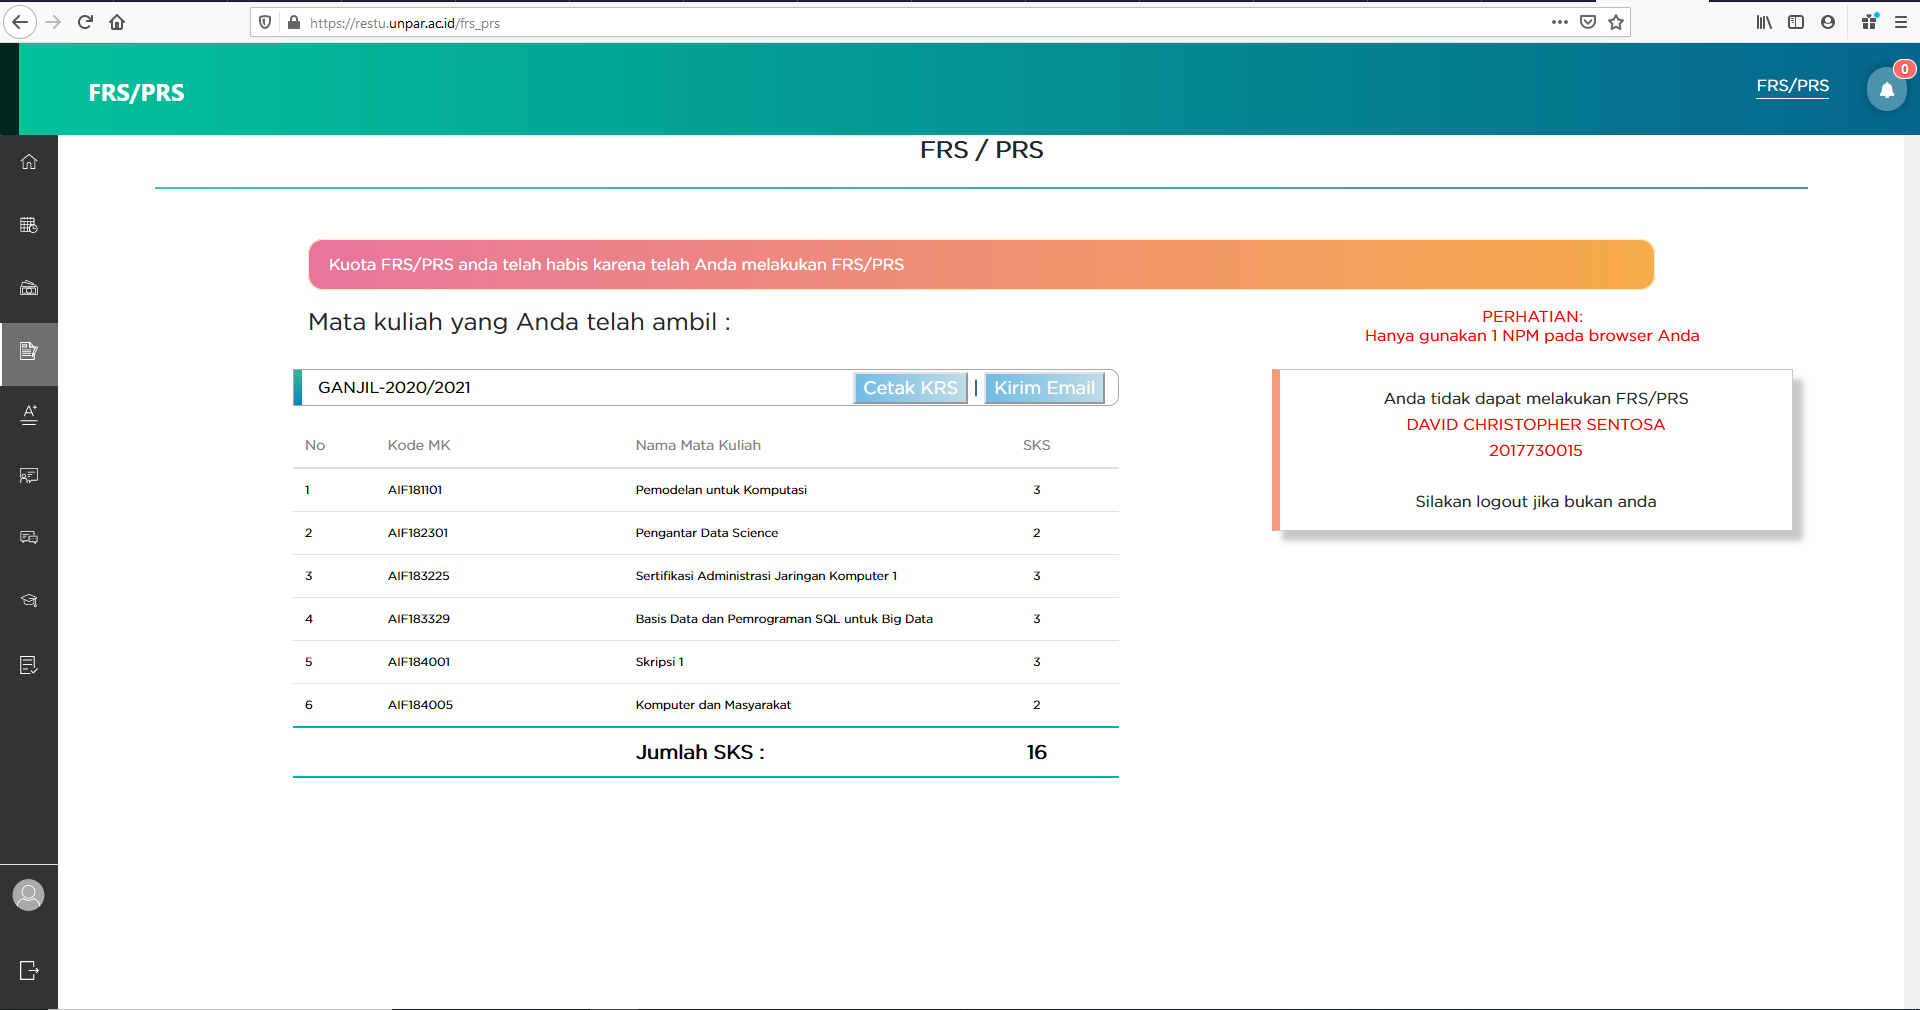
\includegraphics[scale=0.3]{DokumenSkripsi/Gambar/frs.PNG}
				\caption{Tampilan halaman FRS/PRS} 
				\label{fig:pam_frs}
			\end{figure}
    \item \textit{Profil Mahasiswa} : 
    Mahasiswa dapat melihat informasi data diri di halaman profil mahasiswa.
    \begin{itemize}
			\item Nama: Profil mahasiswa
			\item Aktor: Mahasiswa
			\item Deskripsi: Melihat data diri mahasiswa
			\item Kondisi awal: Mahasiswa sudah \textit{login} ke Portal Akademik Mahasiswa
			\item Kondisi akhir: Mahasiswa disajikan informasi data diri
			\item Skenario utama: \\ \\
        \begin{tabular}{|p{0.5cm} |p{6cm}| p{6cm}|}
        \hline
            No & Aksi Aktor &  Reaksi Sistem \\ \hline     
            1 & Mahasiswa menekan tombol profil mahasiswa & Sistem menampilkan halaman profil mahasiswa \\ \hline 
        \end{tabular}
    \end{itemize}
     \begin{figure}[H]
				\centering
				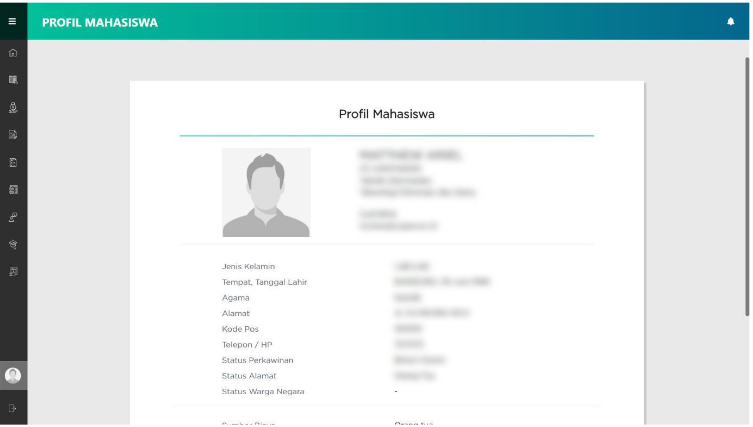
\includegraphics[scale=0.7]{DokumenSkripsi/Gambar/profil}
				\caption{Tampilan halaman profil mahasiswa} 
				\label{fig:pam_profil}
			\end{figure}
	 \item \textit{Pembayaran} : 
    Mahasiswa dapat melihat informasi tentang tagihan pembayaran, riwayat pembayaran, dan keterangan tata cara pembayaran.
    \begin{itemize}
			\item Nama: Profil mahasiswa
			\item Aktor: Mahasiswa
			\item Deskripsi: Melihat informasi pembayaran
			\item Kondisi awal: Mahasiswa sudah \textit{login} ke Portal Akademik Mahasiswa
			\item Kondisi akhir: Mahasiswa disajikan informasi pembayaran
			\item Skenario utama: \\ \\
        \begin{tabular}{|p{0.5cm} |p{6cm}| p{6cm}|}
        \hline
            No & Aksi Aktor &  Reaksi Sistem \\ \hline     
            1 & Mahasiswa menekan tombol pembayaran & Sistem menampilkan halaman pembayaran \\ \hline 
        \end{tabular}
    \end{itemize}
     \begin{figure}[H]
				\centering
				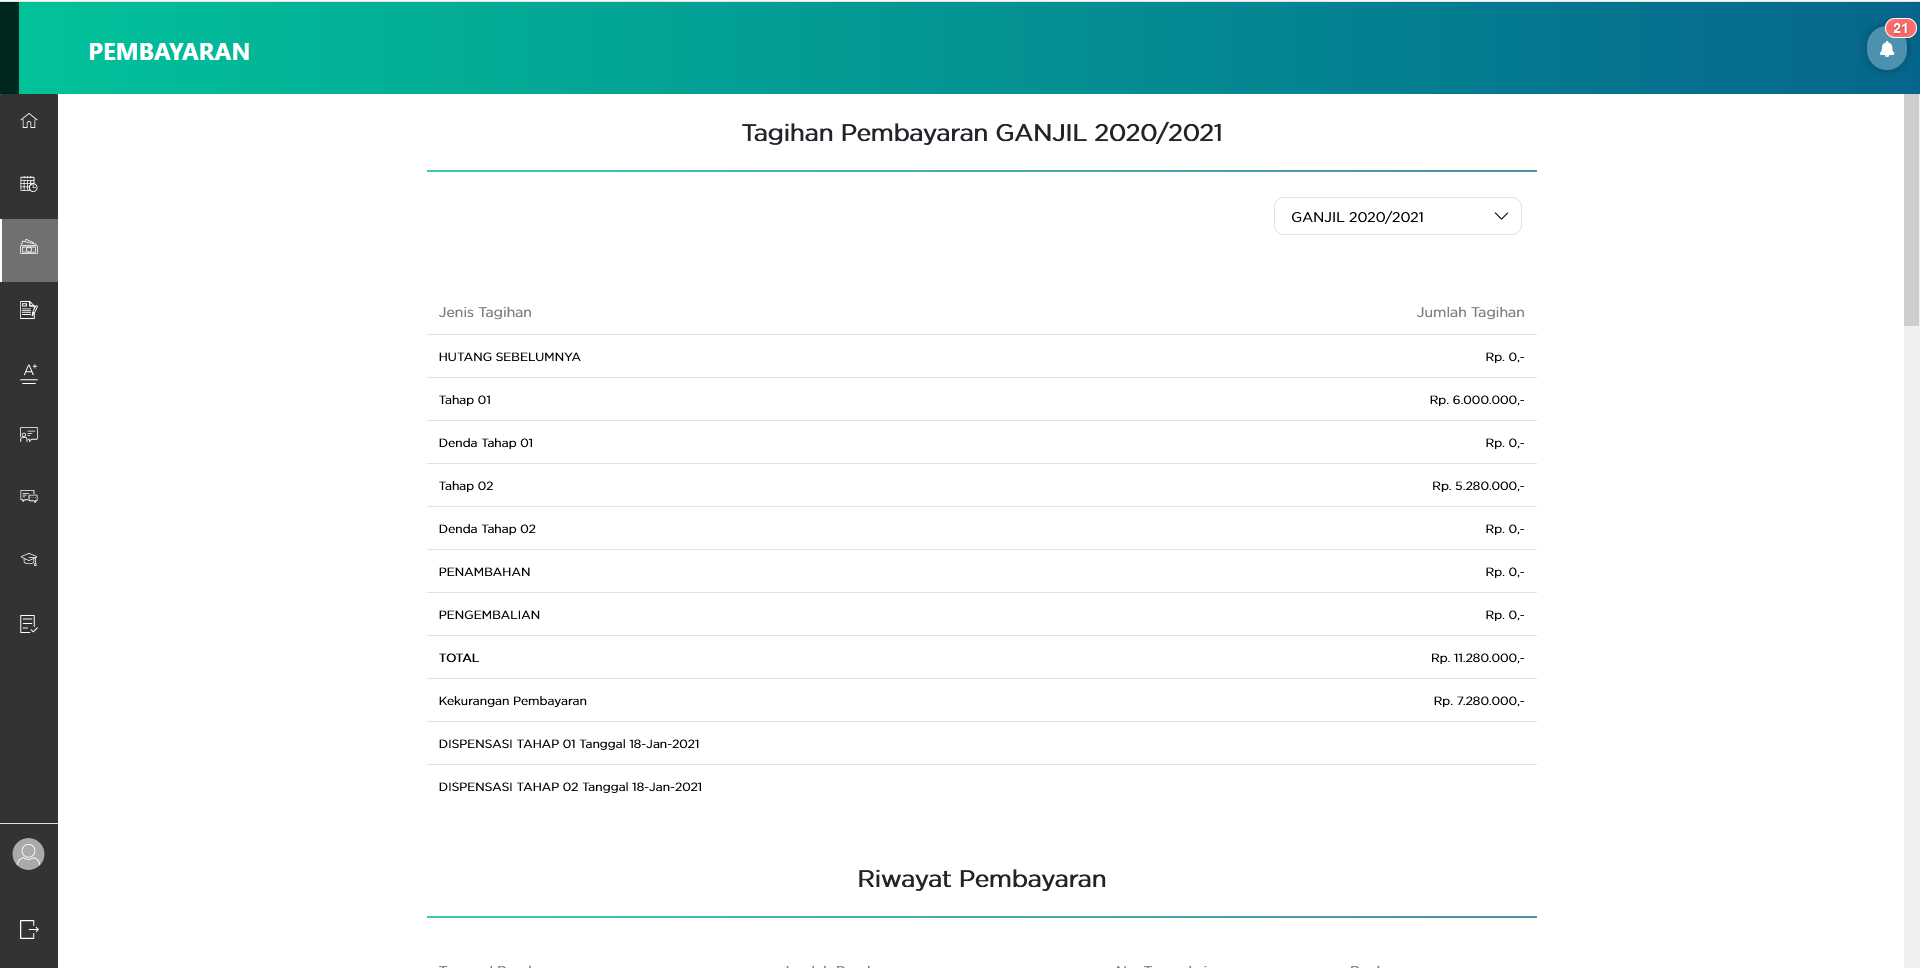
\includegraphics[scale=0.3]{DokumenSkripsi/Gambar/pembayaran}
				\caption{Tampilan halaman pembayaran} 
				\label{fig:pam_pembayaran}
			\end{figure}
    \item \textit{Nilai} : 
    Mahasiswa dapat melihat informasi nilai mata kuliah yang diambil mahasiswa untuk setiap semesternya. Informasi nilai yang tersedia antara lain nilai tugas, angka rata-rata tugas (ART), ujian tengah semester (UTS), ujian akhir semester (UAS), dan TOEFL. Mahasiswa juga bisa melihat grafik perkembangan indeks prestasi kumulatif (IPK) dan indeks prestasi semester (IPS).
    \begin{itemize}
			\item Nama: Profil mahasiswa
			\item Aktor: Mahasiswa
			\item Deskripsi: Melihat informasi nilai 
			\item Kondisi awal: Mahasiswa sudah \textit{login} ke Portal Akademik Mahasiswa
			\item Kondisi akhir: Mahasiswa disajikan informasi nilai
			\item Skenario utama: \\ \\
        \begin{tabular}{|p{0.5cm} |p{6cm}| p{6cm}|}
        \hline
            No & Aksi Aktor &  Reaksi Sistem \\ \hline     
            1 & Mahasiswa menekan tombol nilai & Sistem menampilkan halaman nilai \\ \hline 
        \end{tabular}
    \end{itemize}
     \begin{figure}[H]
				\centering
				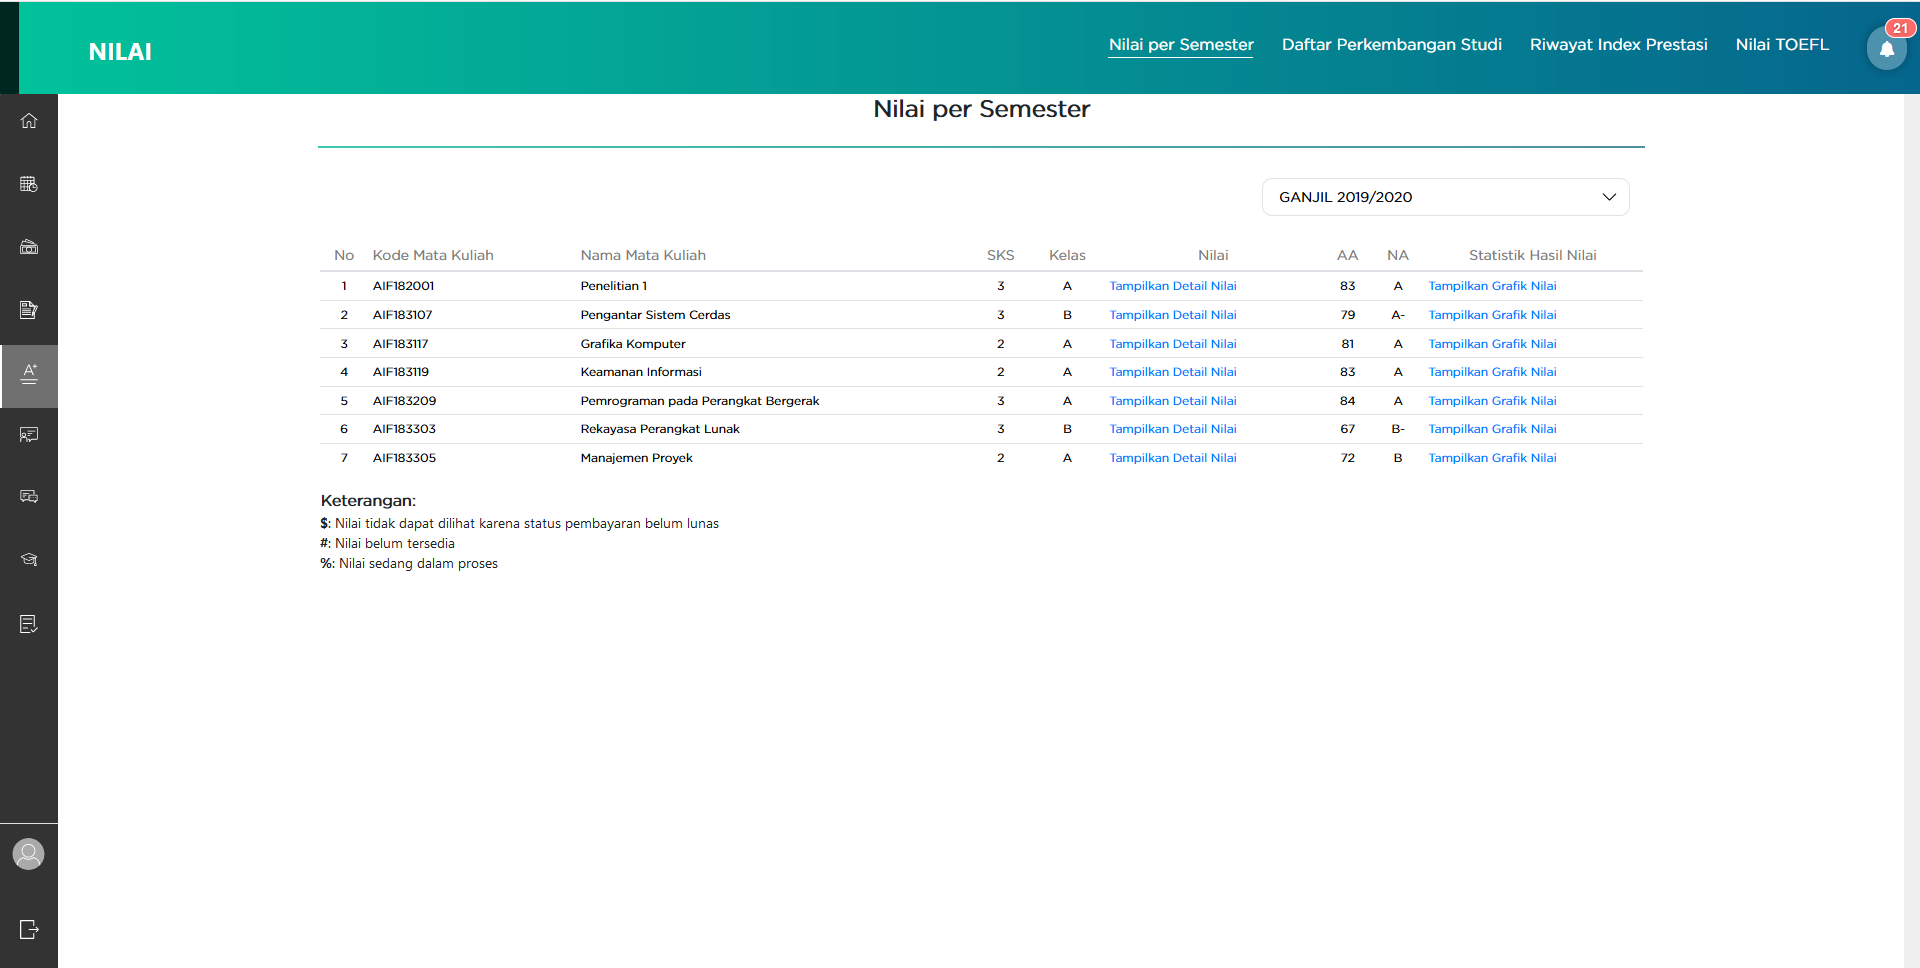
\includegraphics[scale=0.3]{DokumenSkripsi/Gambar/nilai}
				\caption{Tampilan halaman nilai} 
				\label{fig:pam_nilai}
			\end{figure}
			\begin{figure}[H]
				\centering
				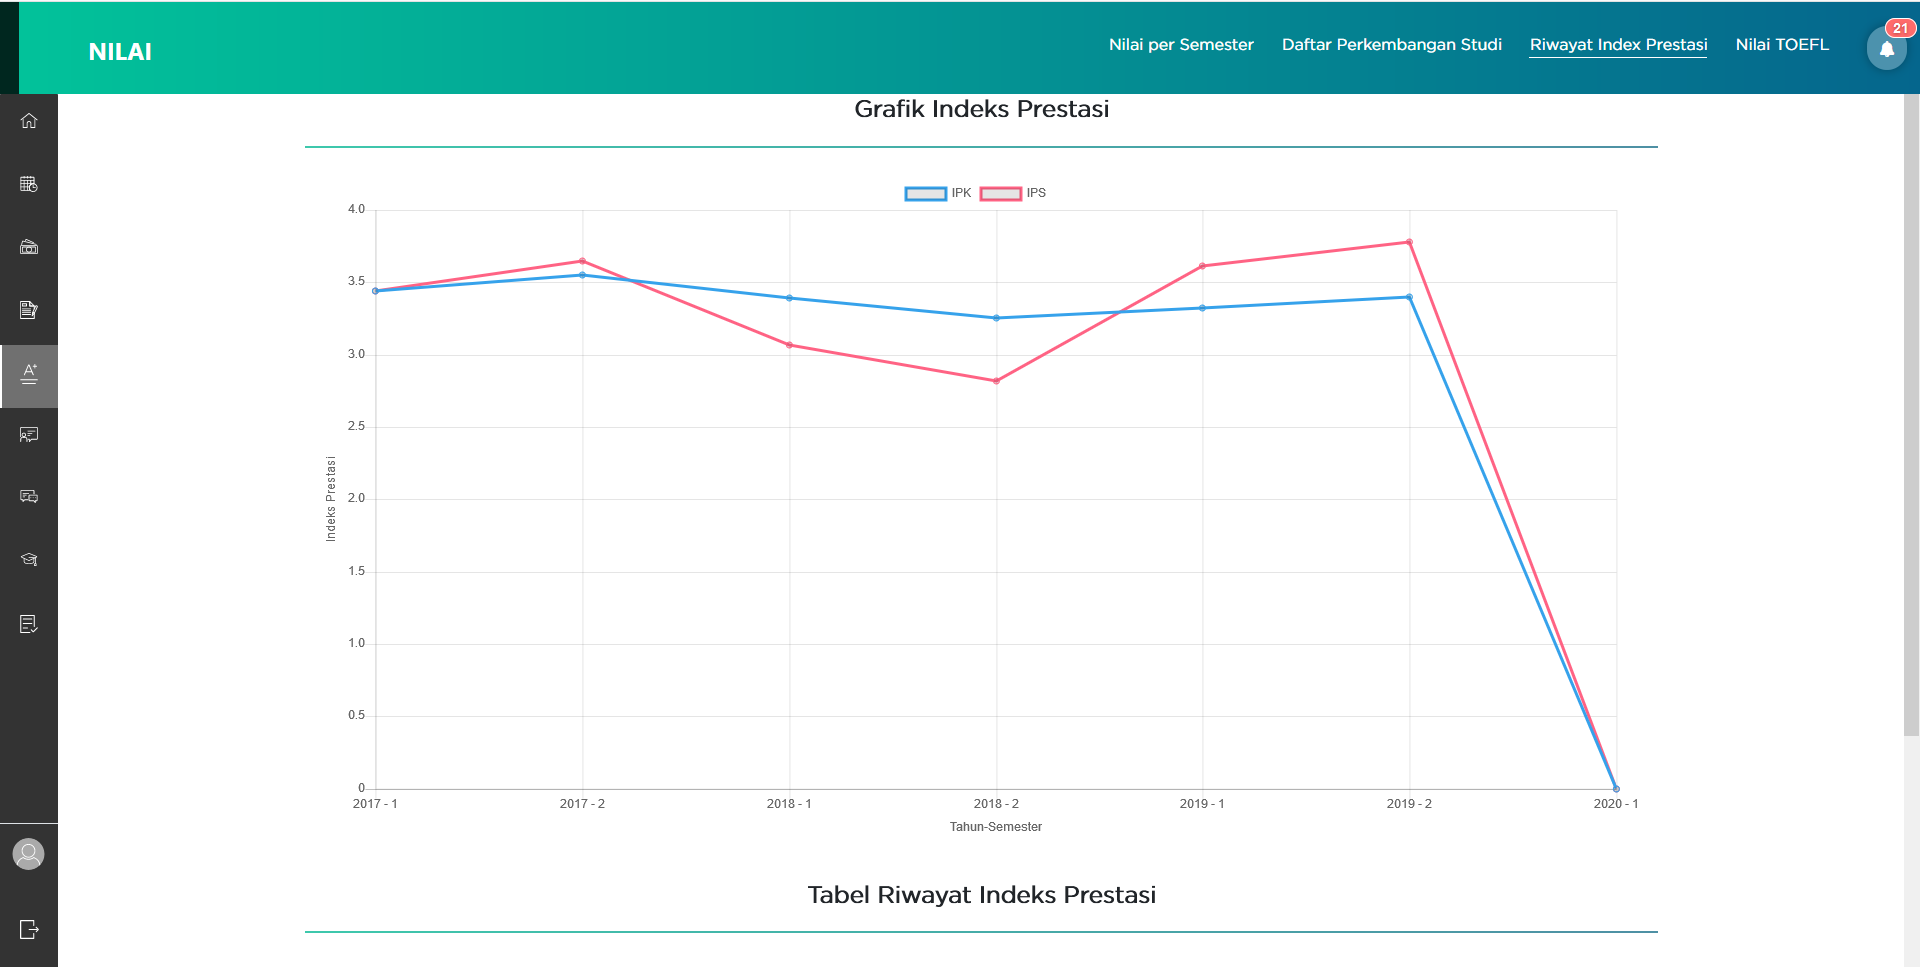
\includegraphics[scale=0.3]{DokumenSkripsi/Gambar/ipk}
				\caption{Tampilan halaman indeks prestasi} 
				\label{fig:pam_ipk}
			\end{figure}
\end{enumerate}

\section{\textit{Jsoup}}
\label{sec:jsoup}
Jsoup adalah \textit{library} Java yang digunakan untuk mengambil data berupa HTML dari sebuah situs. Data HTML tersebut bisa digunakan untuk memperoleh informasi yang diperlukan dari suatu situs\cite{jsoup}. \textit{Library jsoup} ini bisa digunakan saat sebuah situs tidak menyediakan API untuk memberikan datanya. Kelas-kelas yang digunakan dari \textit{library} ini akan dijelaskan di sub bab berikut.

\subsection{Jsoup}
Kelas ini merupakan kelas utama dalam \textit{library} jsoup. Seluruh \textit{method} dalam kelas ini adalah \texttt{static} \textit{method} sehingga kelas ini tidak perlu dikonstruksi terlebih dahulu sebelum menggunakan \textit{method} dari kelas ini. Salah satu \textit{method} yang dimiliki kelas ini adalah sebagai berikut:
\begin{itemize}
	\item \textbf{public static Connection connect(String url)} \\
		Berfungsi untuk membuat koneksi baru dengan suatu situs web. \\
		\textbf{Parameter:}
		\begin{itemize}
			\item \textbf{url} : URL situs web dengan protokol HTTP atau HTTPS.
		\end{itemize}
		\textbf{Kembalian:} koneksi dengan situs web.
\end{itemize}

\subsection{Connection}
Kelas ini merupakan \texttt{interface} yang berguna untuk pengambilan data dari situs web. Beberapa \textit{method} yang dimiliki kelas ini adalah sebagai berikut:

\begin{itemize}
	\item \textbf{Connection cookies(Map<String,String> cookies)} \\
		Berfungsi untuk menambahkan \textit{cookie}. \\
		\textbf{Parameter:}
		\begin{itemize}
			\item \textbf{cookies} : \texttt{Map} dari \textit{cookie}.
		\end{itemize}
		\textbf{Kembalian:} koneksi yang sama tetapi sudah diberi \textit{cookies}.
		
		\item \textbf{Connection data(String key, String value)} \\
		Berfungsi untuk menambahkan parameter data yang bisa dikirim melalui metode HTTP GET atau POST. \\
		\textbf{Parameter:}
		\begin{itemize}
			\item \textbf{key} : kunci data.
			\item \textbf{value} : nilai data.
		\end{itemize}
		\textbf{Kembalian:} koneksi yang sama tetapi sudah diberi parameter data.
		
		\item \textbf{Connection method(Connection.Method method)} \\
		Berfungsi untuk mengatur metode permintaan HTTP, GET atau POST. Metode pengiriman secara \textit{default} adalah GET\\
		\textbf{Parameter:}
		\begin{itemize}
			\item \textbf{method} : metode pengiriman permintaan HTTP.
		\end{itemize}
		\textbf{Kembalian:} koneksi yang sama tetapi sudah diatur metode permintaannya.
		
		\item \textbf{Connection timeout(int millis)} \\
		Berfungsi untuk mengatur batas waktu \textit{request}. Batas waktu nol akan dianggap sebagai batas waktu yang tak terhingga. \\
		\textbf{Parameter:}
		\begin{itemize}
			\item \textbf{millis} : batas waktu dalam milidetik.
		\end{itemize}
		\textbf{Kembalian:} koneksi yang sama tetapi sudah diberi batas waktu untuk \textit{request}.
		
		\item \textbf{Connection validateTLSCertificates(boolean value)} \\
		Berfungsi untuk mengatur pemeriksaan sertifikat TLS untuk permintaan HTTPS. Nilai \texttt{true} untuk memeriksa dan nilai \texttt{false} untuk tidak memeriksa.\\
		\textbf{Parameter:}
		\begin{itemize}
			\item \textbf{value} : status pemeriksaan sertifikat TLS.
		\end{itemize}
		\textbf{Kembalian:} koneksi yang sama tetapi sudah diatur pemeriksaan sertifikatnya.
		
		\item \textbf{Connection.Response execute()} \\
		Berfungsi untuk mengirim permintaan HTTP.\\
		\textbf{Kembalian:} objek \texttt{Response}.	
\end{itemize}

\subsection{Response}

Kelas ini merepresentasikan permintaan HTTP. Beberapa \textit{method} yang dimiliki kelas ini adalah sebagai berikut:
\begin{itemize}
	\item \textbf{Map<String,String> cookies()} \\
		\textit{Method} ini berfungsi untuk mendapatkan seluruh \textit{cookies}. \\
		\textbf{Kembalian:} seluruh \textit{cookies}.	
		
		\item \textbf{Document parse()} \\
		Berfungsi untuk merubah \textit{body} jawaban menjadi dokumen. \\
		\textbf{Kembalian:} dokumen yang sudah dirubah.
		
		\item \textbf{String body()} \\
		Berfungsi untuk mendapatkan \textit{body} jawaban dalam bentuk \textit{string}. \\
		\textbf{Kembalian:} \textit{body} jawaban dalam bentuk \textit{string}.
\end{itemize}

\subsection{Document}

Kelas ini merepresentasikan dokumen HTML. Salah satu \textit{method} yang dimiliki kelas ini adalah sebagai berikut:
\begin{itemize}
	\item \textbf{public Elements select(String cssQuery)} \\
		\textit{Method} ini diturunkan dari kelas Element, berfungsi untuk menemukan elemen HTML yang sesuai dengan kueri CSS. \\
		\textbf{Parameter:} 
		\begin{itemize}
			\item \textbf{cssQuery} : kueri CSS berupa CSS Selector.
		\end{itemize}
		\textbf{Kembalian:} elemen-elemen HTML yang sesuai dengan kueri CSS.	
\end{itemize}

\subsection{Elements}

Kelas ini merepresentasikan kumpulan elemen HTML. Beberapa \textit{method} yang dimiliki kelas ini adalah sebagai berikut:
\begin{itemize}
	\item \textbf{public Elements select(String query)} \\
		Berfungsi untuk menemukan elemen-elemen yang sesuai dalam \textit{list} elemen. \\
		\textbf{Parameter:} 
		\begin{itemize}
			\item \textbf{query} : kueri CSS berupa CSS Selector.
		\end{itemize}
		\textbf{Kembalian:} elemen-elemen yang sudah diseleksi sesuai kueri.	
		
		\item \textbf{public String val()} \\
		Berfungsi untuk mendapatkan nilai dari elemen pertama. \\
		\textbf{Kembalian:} nilai elemen.	
		
		\item \textbf{public String text()} \\
		\textit{Method} Berfungsi untuk mendapatkan kombinasi teks dari seluruh elemen yang sesuai. \\
		\textbf{Kembalian:} seluruh teks dalam \textit{string}.	
\end{itemize}

\subsection{Element}

Kelas ini merepresentasikan sebuah elemen HTML yang berisikan \textit{tag}, atribut, dan anak elemen. Beberapa \textit{method} yang dimiliki kelas ini adalah sebagai berikut:
\begin{itemize}
	\item \textbf{public Element child(int index)} \\
		Berfungsi untuk mendapatkan anak elemen berdasarkan nomor index. \\
		\textbf{Parameter:} 
		\begin{itemize}
			\item \textbf{index} : nomor index.
		\end{itemize}
		\textbf{Kembalian:} anak elemen.	
		
		\item \textbf{public Element children()} \\
		Berfungsi untuk mendapatkan seluruh anak elemen. \\
		\textbf{Kembalian:} seluruh anak elemen.	
		
		\item \textbf{public String className()} \\
		Berfungsi untuk mendapatkan nama kelas elemen. \\
		\textbf{Kembalian:} nama kelas elemen.	
		
		\item \textbf{public String text()} \\
		Berfungsi untuk mendapatkan teks dari elemen. \\
		\textbf{Kembalian:} teks dalam \textit{string}.	
\end{itemize}

\section{SIA Models versi 5.0.0}
SIA Models merupakan \textit{library} Java yang merepresentasikan Sistem Informasi Akademik Teknik Informatika UNPAR \cite{siamodels}. Saat ini SIAModels mendukung kurikulum 2018. Kelas-kelas yang digunakan dari \textit{library} ini akan dijelaskan di sub bab berikut.

\subsection{Mahasiswa}
Kelas ini merepresentasikan seorang mahasiswa Universitas Katolik Parahyangan. Kelas ini memiliki atribut antara lain nama, npm, tanggal lahir, jenis kelamin, riwayat nilai, foto, dan jadwal kuliah. Beberapa \textit{method} yang dimiliki kelas ini adalah sebagai berikut:

\begin{itemize}
	\item \textbf{public byte[] getPhotoImage() throws IOException, MalformedURLException} \\
		Berfungsi untuk mendapatkan foto profil mahasiswa dalam bentuk \textit{byte array}. \\
		\textbf{Kembalian:} \textit{byte array} foto profil mahasiswa.	
		
		\item \textbf{public double calculateIPK() throws ArrayIndexOutOfBoundsException} \\
		Berfungsi untuk menghitung nilai index Prestasi Kumulatif mahasiswa. \\
		\textbf{Kembalian:} nilai IPK mahasiswa.	
		
		\item \textbf{public double calculateIPS(TahunSemester tahunSemester) throws ArrayIndexOutOfBoundsException} \\
		Berfungsi untuk menghitung nilai index Prestasi Semester mahasiswa. \\
		\textbf{Parameter:} 
		\begin{itemize}
			\item \textbf{tahunSemester} : tahun dan semester yang ingin dihitung IPS-nya.
		\end{itemize}
		\textbf{Kembalian:} nilai IPK mahasiswa pada tahun dan semester yang ditentukan.	
		
		\item \textbf{public int calculateSKSTempuh(boolean lulusSaja) throws ArrayIndexOutOfBoundsException} \\
		Berfungsi untuk Menghitung jumlah SKS tempuh mahasiswa saat ini. \\
		\textbf{Parameter:} 
		\begin{itemize}
			\item \textbf{lulusSaja} : set \textit{true} untuk menghitung hanya SKS yang lulus.
		\end{itemize}
		\textbf{Kembalian:} jumlah SKS yang sudah ditempuh mahasiswa.	
\end{itemize}

\subsection{Nilai}
Kelas ini merepresentasikan nilai sebuah mata kuliah mahasiswa Universitas Katolik Parahyangan. Kelas ini memiliki atribut antara lain mata kuliah, kelas, nilai UTS, nilai UAS, dan nilai akhir. Beberapa \textit{method} yang dimiliki kelas ini adalah sebagai berikut:

\begin{itemize}
	\item \textbf{public Double getAngkaAkhir()} \\
		Berfungsi untuk mendapatkan angka akhir dari index nilai. \\
		\textbf{Kembalian:} angka akhir dari nilai.	
\end{itemize}

\subsection{Mata Kuliah}
Kelas ini merepresentasikan sebuah mata kuliah. Kelas ini memiliki atribut antara lain nama, kode, dan sks.

\subsection{Kelulusan}
Kelas ini merepresentasikan kelulusan mahasiswa Universitas Katolik Parahyangan. Kelas ini memiliki atribut daftar mata kuliah wajib lulus sebagai syarat kelulusan. Beberapa \textit{method} yang dimiliki kelas ini adalah sebagai berikut:

\begin{itemize}
	\item \textbf{public boolean checkPrasyarat(Mahasiswa mahasiswa, List<String> reasonsContainer)} \\
		Berfungsi untuk memeriksa apakah mahasiswa sudah memenuhi syarat kelulusan. \\
		\textbf{Parameter:} 
		\begin{itemize}
			\item \textbf{mahasiswa} : mahasiswa yang ingin diperiksa prasyarat kelulusannya.
			\item \textbf{reasonsContainer} : daftar alasan-alasan yang membuat tidak lulus.
		\end{itemize}
		\textbf{Kembalian:} nilai \textit{boolean true} atau \textit{false} yang merepresentasikan status kelulusan prasyarat mahasiswa.	
	\item \textbf{public Map<String, String> getMkEkivalensi()}\\
	    Berfungsi menambahkan data mata kuliah kurikulum 2013 yang ekivalen dengan mata kuliah kurikulum 2018. \\
	    \textbf{Kembalian:} daftar mata kuliah yang ekivalen dengan kurikulum 2018 dalam bentuk \textit{map.}
\end{itemize}

\subsection{Tahun Semester}
Kelas ini merepresentasikan tahun dan semester masa studi mahasiswa di Universitas Katolik Parahyangan. Kelas ini memiliki atribut kode tahun semester yang memiliki 3 dijit dimana 2 dijit pertama adalah tahun dan dijit terakhir adalah kode semester (1 untuk ganjil, 2 untuk genap, 4 untuk pendek). Beberapa \textit{method} yang dimiliki kelas ini adalah sebagai berikut:

\begin{itemize}
    \item \textbf{private static void validateKodeSemester(String kodeTahunSemester) throws IllegalArgumentException} \\
		Berfungsi untuk memvalidasi kode tahun semester. \\
		\textbf{Parameter:} 
		\begin{itemize}
			\item \textbf{kodeTahunSemester} : kode tahun semester yang akan divalidasi.
		\end{itemize}
		\textbf{Eksepsi:} kode semester tidak valid.
\end{itemize}

\section{\textit{Android Design}}
\label{sec:android design}
Dalam mengembangkan aplikasi \textit{Android}, ada pedoman desain yang diberikan. Desain tampilan aplikasi \textit{Android} mengacu pada \textit{Android Material Design}. Pedoman kualitas aplikasi juga diberikan untuk aspek kompatibilitas, keamanan, performa, dll. Kedua pedoman ini diberikan agar aplikasi yang dihasilkan bisa memiliki tampilan dan perilaku yang konsisten dengan platform \textit{Android}. 
 
\subsection{\textit{Material Design}}
\textit{Material Design} terdiri dari panduan, komponen, dan alat-alat untuk mendukung pembuatan tampilan antarmuka yang baik. \textit{Material Design} bertujuan mempermudah kolaborasi antara desainer dan pengembang aplikasi untuk membuat produk yang cantik dengan cepat\cite{materialdesign}. Ada 2 panduan utama yang harus diikuti dari \textit{Material Design} yaitu panduan aksesibilitas dan panduan platform. 

\subsubsection{Panduan Aksesibilitas}
Aksesibilitas dapat diartikan sebagai tingkat kemudahan saat pengguna mempelajari dan menggunakan tampilan antarmuka aplikasi. Meningkatkan aksesibilitas akan meningkatkan \textit{usability} atau tingkat kebergunaan aplikasi kepada berbagai kalangan pengguna \cite{materialdesign}. Hal penting yang harus diperhatikan agar aplikasi memiliki aksesibilitas yang baik :
\begin{itemize}
    \item (HR-01) Hierarki : Elemen-elemen harus terlihat dengan jelas baik dari ukuran, kontras, dan infromasi yang terkandung di dalamnya. Elemen-elemen juga harus terurut berdasarkan kepentingan dan elemen dengan fungsi tertentu diletakan di tempat yang mudah dijangkau.
    \item (WK-01) Warna dan Kontras : Kontras yang cukup tinggi akan membuat elemen terlihat jelas, namun jika terlalu tinggi juga akan kurang nyaman dilihat terlalu lama, jika terlalu rendah maka elemen-elemen akan sulit dibedakan satu sama lain (misal warna teks dengan latar belakangnya). Jika warna digunakan sebagai suatu indikator, maka perlu ada tambahan keterangan lain agar pengguna yang menderita buta warna tetap bisa menerima informasi dengan baik.
    \item (TL-01) Tata Letak dan Tipografi : Menggunakan \textit{layout} yang fleksibel dan resposif akan membantu isi konten menyesuaikan dengan skala layar agar konten tidak ada yang terpotong dengan tidak sengaja. Pastikan menggunakan format sp untuk ukuran \textit{font} agar ukuran teks ikut terskala dengan baik jika pengguna merubah ukuran \textit{font} dari pengaturan sistem perangkat. Pastikan juga ada ruang yang cukup untuk menampung ukuran teks yang diperbesar.
    \item (GB-01) Gambar : Gunakan gambar untuk memperjelas informasi yang disajikan. Gambar logo boleh tidak mematuhi panduan warna, kontras, dan ukuran teks, namun sebaiknya tetap memiliki fungsi (misalnya logo sebagai tombol ke halaman utama).  
\end{itemize}

\subsubsection{Panduan Platform}
Panduan platform membantu menentukan bagaimana ketentuan yang akan digunakan untuk setiap platform. Platform yang dimaksud pada bagian ini adalah bagian-bagian dari komponen aplikasi Android. Platform yang dimaksud adalah :
\begin{itemize}
    \item (NT-01) Notifikasi : notifikasi digunakan untuk memberi tahu komunikasi dari pengguna lain dan mengingatkan hal yang perlu dilakukan. Notifikasi bisa ditampilkan di halaman terkunci, di \textit{status bar}, dengan kedipan lampu LED, dan dengan suara dan getaran. Sebaiknya notifikasi tidak digunakan untuk promosi, meminta rating aplikasi, dan memberi tahu proses yang tidak berhubungan dengan pengguna. Pada saat layar terkunci sebaiknya notifikasi tidak menampilkan informasi yang sensitif. Notifikasi harus punya bagian \textit{header}, bagian konten, dan bagian aksi. 
    \item (IA-01) Izin Akses (\textit{permission}) : Secara normal, aplikasi punya izin akses ke beberapa hal tanpa perlu memintanya kepada pengguna. Namun beberapa hal berikut membutuhkan konfirmasi dari pengguna agar aplikasi memiliki izin akses :
    \begin{itemize} \label{subs:izin}
        \item Kalender : Mengakses dan mengatur kalender.
        \item Kamera : Mengambil foto dan merekam video.
        \item Kontak : Membaca dan mengatur kontak.
        \item Lokasi : Membaca lokasi perangkat saat ini.
        \item Mikrofon : Merekam suara.
        \item Telepon : Membuat dan mengatur panggilan telepon.
        \item Sensor tubuh : Membaca detak jantung dan hal sejenis lainnya.
        \item Media penyimpanan : Mengakses dan menggunakan media penyimpanan.
        \item SMS : Mengirim dan membaca SMS (pesan singkat).
    \end{itemize}
\end{itemize}

\subsection{Kualitas Aplikasi}
Pengguna tentu menginginkan aplikasi berkualitas. Kualitas aplikasi akan menentukan keberhasilan aplikasi dalam hal instalasi, ulasan, loyalitas dan keterlibatan pengguna untuk jangka panjang \cite{androiddesign}. Dokumentasi \textit{Android Developers} memberikan kriteria untuk mengukur kualitas aplikasi sebagai berikut :
\begin{itemize}
    \item Desain visual dan interaksi pengguna
    \item Fungsionalitas
    \item Kompatibilitas, performa, dan stabilitas
    \item Keamanan   
    \item \textit{Google Play}
\end{itemize}
Untuk keterangan lebih lanjut dari setiap poin diatas akan dijelaskan di bagian berikutnya.

\subsubsection{Desain Visual dan Interaksi Pengguna}
Kriteria ini bertujuan memastikan aplikasi akan memiliki desain visual dan pola interaksi standar agar pengalaman pengguna konsisten dan intuitif\cite{androiddev}. Kriteria ini dapat dijabarkan sebagai berikut : 
\begin{itemize}
    \item (UX-B1) Aplikasi tidak boleh merubah definisi ikon sistem dengan fungsinya, jika aplikasi menyediakan ikon yang disesuaikan, maka tampilannya harus mirip ikon standar dan memicu perilaku sesuai fungsi standarnya. 
    \item (UX-S2) Aplikasi hanya menggunakan notifikasi untuk memberitahu perubahan yang terjadi dengan konteks yang berkaitan dengan pengguna pribadi dan untuk memberi tahu informasi/kontrol terhadap kejadian yang sedang berlangsung.
\end{itemize}

\subsubsection{Fungsionalitas}
Kriteria ini bertujuan memastikan aplikasi memberikan perilaku fungsional yang diharapkan, dengan tingkat izin yang sesuai \cite{androiddev}. Kriteria ini dapat dijabarkan sebagai berikut : 
\begin{itemize}
    \item (FN-P1) Aplikasi hanya meminta izin untuk mendukung fungsionalitas aplikasi tersebut. Aplikasi tidak boleh meminta izin untuk mengakses data sensitif atau menggunakan layanan yang bisa membebani pengguna kecuali jika fitur inti aplikasi memerlukan izin tersebut.
    \item (FN-L1) Aplikasi harus berfungsi normal jika dipasang di kartu \textit{SD}.
    \item (FN-A1) Audio tidak boleh diputar di layar utama, saat layar mati, dibalik layar, atau saat layar dikunci kecuali memutar audio adalah fitur utama.
    \item (FN-U1) Jika memungkinkan aplikasi mendukung orientasi \textit{landscape} dan \textit{portrait}, dan menggunakan seluruh layar untuk kedua orientasi.
    \item (FN-S1) Aplikasi tidak boleh membiarkan layanan tetap aktif saat di latar belakang layar, kecuali jika diperlukan fitur utama.
    \item (FN-S2) Aplikasi mempertahankan status pengguna atau aplikasi saat meninggalkan latar depan dan mencegah kehilangan data tanpa sengaja akibat navigasi mundur dan perubahan status lainnya. 
\end{itemize}

\subsubsection{Kompatibilitas, Performa, dan Stabilitas}
Kriteria ini bertujuan memastikan aplikasi memberikan kompatibilitas, performa, stabilitas, dan daya respons yang diharapkan oleh pengguna \cite{androiddev}. Kriteria ini dapat dijabarkan sebagai berikut : 
\begin{itemize}
    \item (PS-S1) Aplikasi diharapkan tidak macet, berfungsi tidak normal, menutup sendiri di perangkat yang menjalankan.
    \item (PS-P1) Aplikasi dimuat dengan cepat atau memberikan indikasi kepada pengguna tentang kapan aplikasi selesai dimuat.
    \item (PS-T1) Aplikasi dibuat dengan \textit{SDK} terbaru dan berjalan di \textit{Android} versi terbaru tanpa kendala.
    \item (PS-M1) Aplikasi memutar video dan audio dengan lancar, tidak tersendat, suara dan gambar tidak pecah, atau cacat lainnya.
    \item (PS-V1) Aplikasi menyediakan grafik berkualitas tinggi untuk semua ukuran layar yang ditargetkan dan menampilkan elemen antarmuka tanpa pikselasi, distorsi, dan tidak bergerigi pada tepian.
    \item (PS-B1) Aplikasi mendukung fitur pengelolaan daya baterai (\textit{Android 6.0+}).  
\end{itemize}   

\subsubsection{Keamanan}
Kriteria ini bertujuan memastikan aplikasi menangani dan mengamankan data pengguna dan informasi pribadi dengan benar\cite{androiddev}. Kriteria ini dapat dijabarkan sebagai berikut :
\begin{itemize}
    \item (SC-D1) Aplikasi harus menyimpan data pribadi di penyimpanan internal aplikasi dan tidak boleh mencatat data pribadi di log.
    \item (SC-D2) Aplikasi harus memverifikasi data eksternal sebelum digunakan.
    \item (SC-P1) Aplikasi hanya boleh mengekspor komponen aplikasi yang membagikan data dengan aplikasi lain, atau komponen yang harus dipanggil oleh aplikasi lain.
    \item (SC-P2) Semua komponen aplikasi yang berbagi konten dengan aplikasi lain menetapkan (dan memberlakukan) izin yang sesuai, termasuk aktivitas, layanan, penerima siaran, dan khususnya penyedia konten.
    \item (SC-N1) Aplikasi harus menyatakan konfigurasi keamanan jaringan dan semua lalu lintas jaringan dilakukan melalui \textit{SSL}.
    \item (SC-N2) Jika aplikasi menggunakan layanan \textit{Google Play}, inisialisasi keamanan dilakukan saat aplikasi dimulai.
    \item (SC-U1) Aplikasi harus menggunakan dependensi, \textit{library} dan \textit{SDK} terbaru.
    \item (SC-E1) Aplikasi tidak boleh menjalankan kode dari luar aplikasi secara dinamis.
    \item (SC-C1) Aplikasi harus menggunakan algoritma kriptografi kuat yang disediakan oleh platform.
\end{itemize}       

\subsubsection{\textit{Google Play}}
Kriteria ini bertujuan memastikan aplikasi yang dibuat sudah layak, memenuhi standar dan syarat untuk dipublikasikan di layanan \textit{Google Play}\cite{androiddev}. Kriteria ini dapat dijabarkan sebagai berikut :
\begin{itemize}
    \item (GP-P1) Aplikasi mematuhi Kebijakan Materi Pengembang \textit{Google Play} (tidak menawarkan materi tidak pantas, tidak menggunakan hak kekayaan intelektual atau merk orang lain, dll).
    \item (GP-D1) Aplikasi sudah memenuhi kriteria yang sudah diuraikan sebelum bagian ini.
    \item (GP-X1) Pengembang aplikasi harus mengatasi \textit{bug} yang disampaikan di halaman ulasan di layanan \textit{Google Play} jika \textit{bug} tersebut ditemukan di banyak perangkat dan berulang kali atau ditemukan di perangkat terbaru atau perangkat paling populer.    
\end{itemize}  


% \subsection{Tabel}  
% Berikut adalah contoh pembuatan tabel. 
% Penempatan tabel dan gambar secara umum diatur secara otomatis oleh \LaTeX{}, perhatikan contoh di file bab2.tex untuk melihat bagaimana cara memaksa tabel ditempatkan sesuai keinginan kita.

% Perhatikan bawa berbeda dengan penempatan judul gambar gambar, keterangan tabel harus diletakkan di atas tabel!!
% Lihat Tabel~\ref{tab:contoh1} berikut ini:

% \begin{table}(H) %atau h saja untuk "kira kira di sini"
% 	\centering 
% 	\caption{Tabel contoh}
% 	\label{tab:contoh1}
% 	\begin{tabular}{cccc}
% 		\toprule
% 		& $v_{start}$ & $\mathcal{S}_{1}$ & $v_{end}$\\

% 		\midrule
% 		$\tau_{1}$ & 1 & 12& 20\\
% 		$\tau_{2}$ & 1 &  & 20\\
% 		$\tau_{3}$ & 1 & 9 & 20\\
% 		$\tau_{4}$ & 1 &  & 20\\

% 		\bottomrule
		
% 	\end{tabular} 
% \end{table}
% Tabel~\ref{tab:cthwarna1} dan Tabel~\ref{tab:cthwarna2} berikut ini adalah tabel dengan sel yang berwarna dan ada dua tabel yang bersebelahan. 
% \begin{table}(H)
% 	\begin{minipage}(c){0.49\linewidth}
% 		\centering
% 		\caption{Tabel bewarna(1)}
% 		\label{tab:cthwarna1}
% 		\begin{tabular}{ccccc}
% 			\toprule
% 			 & $v_{start}$ & $\mathcal{S}_{2}$ & $\mathcal{S}_{1}$ & $v_{end}$\\
			
% 			\midrule
% 			$\tau_{1}$ & 1 & 5 \cellcolor{green}& 12& 20\\
% 			$\tau_{2}$ & 1 & 8 \cellcolor{green}& & 20\\
% 			$\tau_{3}$ & 1 & 2/8/17 \cellcolor{green}& 9 & 20\\
% 			$\tau_{4}$ & 1 & \cellcolor{red}& & 20\\
			
% 			\bottomrule

% 		\end{tabular}
% 	\end{minipage}
% 	\begin{minipage}(c){0.49\linewidth}
		
% 		\centering 
% 		\caption{Tabel bewarna(2)}
% 		\label{tab:cthwarna2}
% 		\begin{tabular}{ccccc}
% 			\toprule
% 			 & $v_{start}$ & $\mathcal{S}_{1}$ & $\mathcal{S}_{2}$ & $v_{end}$\\
			
% 			\midrule
% 			$\tau_{1}$ & 1 & 12& 5 \cellcolor{red} &20\\
% 			$\tau_{2}$ & 1 &  &  8 \cellcolor{green} &20\\
% 			$\tau_{3}$ & 1 & 9 & 2/8/17 \cellcolor{green} &20\\
% 			$\tau_{4}$ & 1 &   & \cellcolor{red} &20\\
			
% 			\bottomrule
		
% 		\end{tabular}
% 	\end{minipage}
% \end{table}

 
% \subsection{Kutipan}
% \label{subs:kutipan} 
% Berikut contoh kutipan dari berbagai sumber, untuk keterangan lebih lengkap, silahkan membaca file referensi.bib yang disediakan juga di template ini.
% Contoh kutipan:
% \begin{itemize}
% 	\item Buku:~\cite{berg:08:compgeom} 
% 	\item Bab dalam buku:~\cite{kreveld:04:GIS}
% 	\item Artikel dari Jurnal:~\cite{buchin:13:median}
% 	\item Artikel dari prosiding seminar/konferensi:~\cite{kreveld:11:median}
% 	\item Skripsi/Thesis/Disertasi:~\cite{lionov:02:animasi}~\cite{wiratma:10:following}~\cite{wiratma:22:later}
% 	\item Technical/Scientific Report:~\cite{kreveld:07:watertight}
% 	\item RFC (Request For Comments):~\cite{RFC1654}
% 	\item Technical Documentation/Technical Manual:~\cite{Z.500}~\cite{unicode:16:stdv9}~\cite{google:16:and7}
% 	\item Paten:~\cite{webb:12:comm}
% 	\item Tidak dipublikasikan:~\cite{wiratma:09:median}~\cite{lionov:11:cpoly}
% 	\item Laman web:~\cite{erickson:03:cgmodel}  
% 	\item Lain-lain:~\cite{agung:12:tango}
% \end{itemize}    
  
% \subsection{Gambar}

% Pada hampir semua editor, penempatan gambar di dalam dokumen \LaTeX{} tidak dapat dilakukan melalui proses {\it drag and drop}.
% Perhatikan contoh pada file bab2.tex untuk melihat bagaimana cara menempatkan gambar.
% Beberapa hal yang harus diperhatikan pada saat menempatkan gambar:
% \begin{itemize}
% 	\item Setiap gambar {\bf harus} diacu di dalam teks (gunakan {\it field} {\sc label})
% 	\item {\it Field} {\sc caption} digunakan untuk teks pengantar pada gambar. Terdapat dua bagian yaitu yang ada di antara tanda $($ dan $)$ dan yang ada di antara tanda $\{$ dan $\}$. Yang pertama akan muncul di Daftar Gambar, sedangkan yang kedua akan muncul di teks pengantar gambar. Untuk skripsi ini, samakan isi keduanya.
% 	\item Jenis file yang dapat digunakan sebagai gambar cukup banyak, tetapi yang paling populer adalah tipe {\sc png} (lihat Gambar~\ref{fig:ularpng}), tipe {\sc jpg} (Gambar~\ref{fig:ularjpg}) dan tipe {\sc pdf} (Gambar~\ref{fig:ularpdf})
% 	\item Besarnya gambar dapat diatur dengan {\it field} {\sc scale}.
% 	\item Penempatan gambar diatur menggunakan {\it placement specifier} (di antara tanda  $($ dan $)$ setelah deklarasi gambar.
% 	Yang umum digunakan adalah {\bf H} untuk menempatkan gambar {\bf sesuai} penempatannya di file .tex atau  {\bf h} yang berarti "kira-kira" di sini. \\
% 	Jika tidak menggunakan {\it placement specifier}, \LaTeX{} akan menempatkan gambar secara otomatis untuk menghindari bagian kosong pada dokumen anda.
% 	Walaupun cara ini sangat mudah, hindarkan terjadinya penempatan dua gambar secara berurutan. 	
% 	\begin{itemize}
% 		\item Gambar~\ref{fig:ularpng} ditempatkan di bagian atas halaman, walaupun penempatannya dilakukan setelah penulisan 3 paragraf setelah penjelasan ini.
% 		\item Gambar~\ref{fig:ularjpg} dengan skala 0.5 ditempatkan di antara dua buah paragraf. Perhatikan penulisannya di dalam file bab2.tex!
% 		\item Gambar~\ref{fig:ularpdf} ditempatkan menggunakan {\it specifier} {\bf h}.
% 	\end{itemize}
% \end{itemize}
 
% \dtext{17-18}
% \begin{figure} 
% 	\centering  
% 	\includegraphics(scale=1){ular-png}  
% 	\caption(Gambar {\it Serpentes} dalam format png){Gambar {\it Serpentes} dalam format png} 
% 	\label{fig:ularpng} 
% \end{figure} 

% \dtext{19-20}
% \begin{figure}(H)
% 	\centering  
% 	\includegraphics(scale=0.5){ular-jpg}  
% 	\caption(Ular kecil){Ular kecil} 
% 	\label{fig:ularjpg} 
% \end{figure} 
% \dtext{21-22}

% \begin{figure}(ht) 
% 	\centering  
% 	\includegraphics(scale=1){ular-pdf}  
% 	\caption( {\it Serpentes} betina){ {\it Serpentes} jantan} 
% 	\label{fig:ularpdf} 
% \end{figure} 
 
